\documentclass{article}
\usepackage[utf8]{inputenc}
\usepackage{graphicx}
% \usepackage{hyperref}
\usepackage[hidelinks]{hyperref}
\usepackage{listings}
\usepackage{color}
\usepackage{xcolor} % Per definire i colori personalizzati
\usepackage{amsmath} % Per formattazione matematica
\usepackage{amssymb}
\usepackage[a4paper, left=1in, right=1in, top=1in, bottom=1in]{geometry}
\usepackage{float}

\lstset{
    basicstyle=\ttfamily\small,
    breaklines=true,
    breakatwhitespace=false,
    prebreak=\raisebox{0ex}[0ex][0ex]{\ensuremath{\char`\\}},
    frame=single,
    showstringspaces=false,
    columns=flexible
}

% Definire un colore personalizzato usando HEX
\definecolor{myblue}{HTML}{003054} % Sostituisci con il tuo colore HEX

\title{Kubernetes Network Policies and Service Meshes Lab}

\date{} % Non visualizzare la data in questo punto

\begin{document}

% Politecnico di Torino in alto al centro, non in grassetto
\begin{center}
  \textnormal{\LARGE Politecnico di Torino} % Titolo grande, normale, non grassetto
\end{center}

% Impostare il titolo con il colore personalizzato al centro
\begin{center}
  \vspace*{6cm} % Spazio verticale dall'inizio della pagina
  {\color{myblue}\Huge \textsf{Kubernetes Network Policies}} % Prima riga del titolo
  
  \vspace{0.5cm} % Spazio verticale tra le righe del titolo
  
  {\color{myblue}\Huge \textsf{and Service Meshes}} % Seconda riga del titolo
  
  % Riga orizzontale colorata
  \vspace{0.5cm} % Spazio tra il titolo e la riga
  \noindent\textcolor{myblue}{\rule{\textwidth}{0.8pt}} % Riga colorata
\end{center}

% Autore in basso
\vspace*{\fill}
\begin{center}
    \large Alessandro Genova \\ % Nome autore
    \large s330893
    \vspace*{0.5cm}
\end{center}

% Spazio per l'immagine del logo
\begin{center}
    
\includegraphics[width=0.3\textwidth]{imgs/polito.eps} % Placeholder per il logo
\end{center}

% Data in fondo alla pagina
\begin{center}
    \vspace*{0.5cm}
    August 2024
\end{center} 

\newpage
\tableofcontents
\newpage

\section{Introduction}
This lab provides aims at practicing with two essential technologies for improving network security and service communication in Kubernetes: Network Policies and Service Meshes. Network Policies control pod-to-pod communication by acting as a firewall, while Service Meshes, such as Istio, manage service-to-service communication, offering features like traffic management, security and observability.
\\\\
By the end of this lab, students will:

\begin{itemize}
    \item Implement and test Kubernetes Network Policies to control pod communication.
    \item Deploy and configure Istio as a Service Mesh.
    \item Apply traffic management using Istio's Virtual Services and Destination Rules.
    \item Implement mutual TLS (mTLS) between services.
    \item Use observability tools like Kiali, Grafana, and Jaeger in Istio.
    \item Understand the different use cases for Network Policies and Service Meshes.
\end{itemize}

\newpage

\section{Lab Environment Setup}

\subsection{Kubernetes Cluster Setup}
Let's start by setting up the necessary tools and environment. 
\\\\
  \textbf{Steps:}
  \begin{enumerate}
      \item \textbf{Install Docker}, instructions at: \footnotesize\url{https://docs.docker.com/engine/install/ubuntu/}.
      \begin{lstlisting}
# Add Docker's official GPG key:
sudo apt-get update
sudo apt-get install ca-certificates curl
sudo install -m 0755 -d /etc/apt/keyrings
sudo curl -fsSL https://download.docker.com/linux/ubuntu/gpg -o /etc/apt/keyrings/docker.asc
sudo chmod a+r /etc/apt/keyrings/docker.asc

# Add the repository to Apt sources:
echo \
  "deb [arch=$(dpkg --print-architecture) signed-by=/etc/apt/keyrings/docker.asc] https://download.docker.com/linux/ubuntu \
  $(. /etc/os-release && echo "$VERSION_CODENAME") stable" | \
  sudo tee /etc/apt/sources.list.d/docker.list > /dev/null

sudo apt-get update
# Install docker
sudo apt-get install -y docker-ce docker-ce-cli containerd.io docker-buildx-plugin docker-compose-plugin

# Add to group to use docker as normal user
sudo usermod -aG docker $USER && newgrp docker

# Verify docker works
docker run hello-world
      \end{lstlisting}
      \normalsize
      \item \textbf{Install Minikube + Cilium}, instructions at:
    \begin{itemize}
        \item \footnotesize\url{https://minikube.sigs.k8s.io/docs/start/?arch=%2Flinux%2Fx86-64%2Fstable%2Fbinary+download}
        \item \footnotesize\url{https://docs.cilium.io/en/stable/gettingstarted/k8s-install-default/}
        \item \footnotesize\url{https://kubernetes.io/docs/tasks/tools/install-kubectl-linux/#install-using-native-package-management}
    \end{itemize}
    For this lab, we'll be using Minikube to set up our Kubernetes cluster. Minikube was chosen for several reasons:

    \begin{itemize}
        \item \textbf{Simplicity and Ease of Use}: Minikube is designed to be easy to install and configure, making it ideal for who is new to Kubernetes or for testing and developing applications in a local environment.
        \item \textbf{Minimal Resources}: Unlike other solutions that require multiple nodes and significant resources, Minikube can run on a single machine with minimal resource requirements (requires only 2GB of free RAM). This makes it perfect for small projects.
    \end{itemize}
    In this lab, for simplicity, we will have only one control node and only one worker node.

      \textbf{Important Note:} It's not sufficient to just install Minikube. To enable Network Policies in your Kubernetes cluster, you need to initialize the cluster with a CNI (Container Network Interface) that supports Network Policies. To enable Network Policies in your Kubernetes cluster, you need to initialize the cluster with a CNI (Container Network Interface) that supports Network Policies. A CNI plugin configures network interfaces for containers and sets up network bridges (which link network segments and manage traffic) on the host. By default, Kubernetes does not support Network Policies unless a CNI is installed. 
      
      After some testing, I found out that \textbf{Cilium} is the CNI that works better in this case (also according to Cloud Computing Polito labs, Cilium is the recommended choice).
      
      You can use the default Kubernetes NetworkPolicy resources with Cilium, or optionally take advantage of the more advanced policies specific for Cilium. We'll concentrate on default Kubernetes ones.
  
      Follow the instructions below to set up Minikube with Cilium as the CNI:
  
      \begin{lstlisting}
sudo apt update && sudo apt install -y curl
# Install minikube
curl -LO https://storage.googleapis.com/minikube/releases/latest/minikube-linux-amd64
sudo install minikube-linux-amd64 /usr/local/bin/minikube && rm minikube-linux-amd64

# If you haven't done it before, add to group to use docker as normal user
sudo usermod -aG docker $USER && newgrp docker

minikube config set driver docker # could be useful to set this, because if we forget to manually specify the driver, docker will be automatically considered

# Start Minikube with Cilium CNI:
minikube delete && minikube start --driver=docker --cni=cilium

# Install kubectl if not already installed:
sudo apt-get update
sudo apt-get install -y apt-transport-https ca-certificates curl gnupg && sudo mkdir -p /etc/apt/keyrings/
curl -fsSL https://pkgs.k8s.io/core:/stable:/v1.31/deb/Release.key | sudo gpg --dearmor -o /etc/apt/keyrings/kubernetes-apt-keyring.gpg
sudo chmod 644 /etc/apt/keyrings/kubernetes-apt-keyring.gpg # allow unprivileged APT programs to read this keyring
echo "deb [signed-by=/etc/apt/keyrings/kubernetes-apt-keyring.gpg] https://pkgs.k8s.io/core:/stable:/v1.31/deb/ /" | sudo tee /etc/apt/sources.list.d/kubernetes.list
sudo chmod 644 /etc/apt/sources.list.d/kubernetes.list   # helps tools such as command-not-found to work correctly
sudo apt-get update
sudo apt-get install -y kubectl
  
      \end{lstlisting}

      % # Install the Cilium CLI (copy from the website docs.cilium.io url above, otherwise the copy-paste will be not correctly formatted):
      % CILIUM_CLI_VERSION=$(curl -s https://raw.githubusercontent.com/cilium/cilium-cli/main/stable.txt)
      % CLI_ARCH=amd64
      % if [ "$(uname -m)" = "aarch64" ]; then CLI_ARCH=arm64; fi
      % curl -L --fail --remote-name-all https://github.com/cilium/cilium-cli/releases/download/${CILIUM_CLI_VERSION}/cilium-linux-${CLI_ARCH}.tar.gz{,.sha256sum}
      % sha256sum --check cilium-linux-${CLI_ARCH}.tar.gz.sha256sum
      % sudo tar xzvfC cilium-linux-${CLI_ARCH}.tar.gz /usr/local/bin
      % rm cilium-linux-${CLI_ARCH}.tar.gz{,.sha256sum}
      
      % # Install Cilium in the Kubernetes cluster:
      % cilium install --version 1.16.1 # IGNORE ERRORS
      % # (Note: The 'cilium install' command might display some warnings or errors, 
      % # but you can ignore them.)
      
      % # (Optional) Test Cilium connectivity:
      % cilium connectivity test 
    

      \item \textbf{Verify Internet Connectivity:}
      After starting Minikube, verify that the cluster has internet connectivity by running the following commands:
      \begin{lstlisting}
minikube ssh
ping google.com
      \end{lstlisting}
      If the ping fails, modify the DNS settings with these steps:
      \begin{lstlisting}
sudo vi -c "set nocompatible" /etc/resolv.conf  # set nocompatible is to make vi similar to vim
      \end{lstlisting}
      In the `vi` editor:
      \begin{itemize}
          \item Press `i` to enter insert mode.
          \item Locate the `nameserver` line, delete the existing IP, and replace it with `8.8.8.8`.
          \item Press `Esc`, then type `:wq` and press `Enter` to save and exit.
      \end{itemize}
      
      Try pinging again. If successful, exit the Minikube node by typing `exit` or by pressing `Ctrl+D`.

      \item \textbf{Minikube Dashboard:}
      To open the Minikube dashboard in your browser, use the following command:
      \begin{lstlisting}
minikube dashboard &        # where '&' is to open in background and be able to continue to use the same terminal
      \end{lstlisting}
      Wait some time and it will output the url to reach we the web dashboard. The dashboard provides a graphical interface to monitor and manage your Kubernetes resources. However, for learning purposes, we recommend using terminal commands instead of relying on the dashboard GUI.

      \begin{figure}[H]
        \centering
        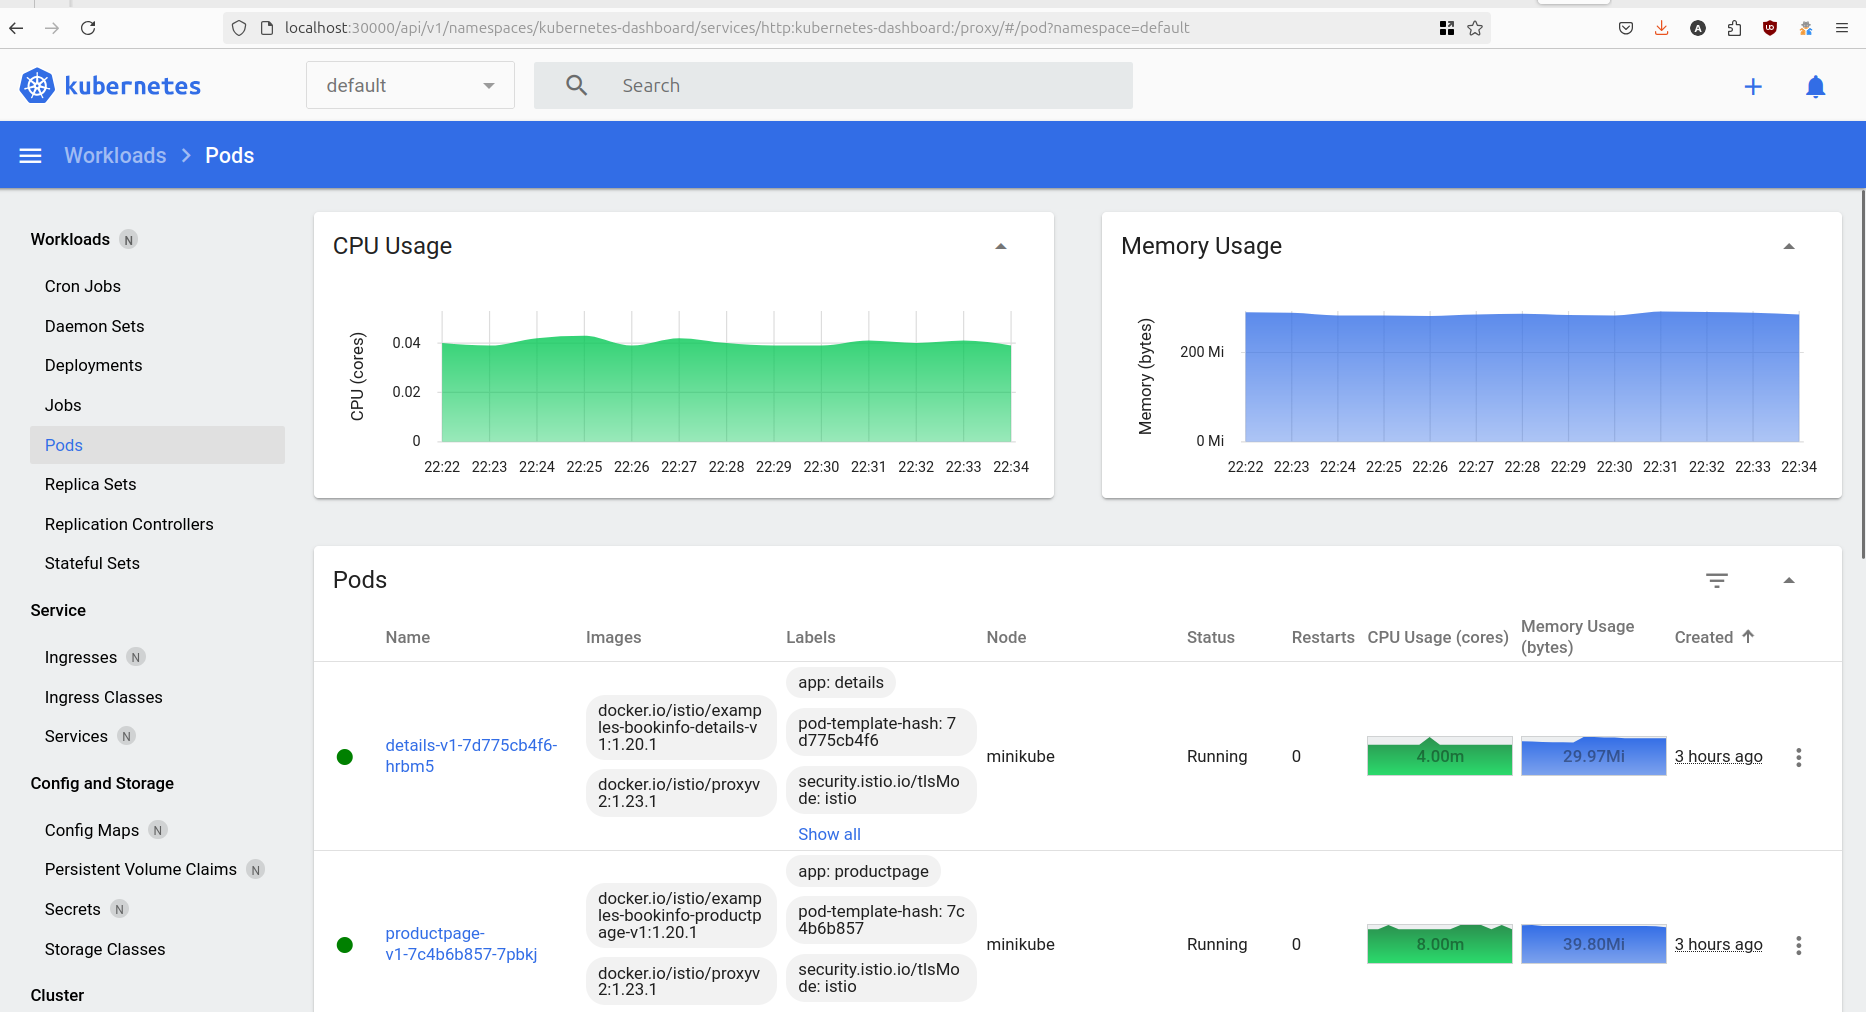
\includegraphics[width=0.8\textwidth]{imgs/webdashboard.eps}
        \caption{Kubernetes Web Dashboard}
    \end{figure}

    To also view CPU and memory usage of your pods (like in the image), you can enable the metrics-server addon. This addon is also necessary to display these metrics via the terminal with `kubectl top pods`:
      \begin{lstlisting}
minikube addons enable metrics-server
      \end{lstlisting}

  \end{enumerate}

\subsection{Remote Access and SSH Tunneling with CrownLabs}

If you are using the CrownLabs service offered by Politecnico di Torino, follow these instructions to access dashboards or applications, running on the remote machine.
\\\\
Assuming you have connected to the CrownLabs machine using the following SSH command, where \texttt{CROWNLABS\_REMOTE\_IP} is the IP address of the CrownLabs machine you have access:
  \begin{lstlisting}
ssh -J bastion@ssh.crownlabs.polito.it crownlabs@CROWNLABS_REMOTE_IP
  \end{lstlisting}

  \textbf{Setting Up an SSH Tunnel:}

  To access web-based services on a remote machine, you can establish an SSH tunnel that forwards traffic from a local port to a service on the CrownLabs machine. Use the following command:
  
  \begin{lstlisting}
  ssh -J bastion@ssh.crownlabs.polito.it crownlabs@CROWNLABS_REMOTE_IP \
      -L LOCAL_PORT:LOCAL_CROWNLABS_MACHINE_ADDRESS:REMOTE_PORT -N &
  \end{lstlisting}
  
  \begin{itemize}
      \item \texttt{LOCAL\_PORT}: The port on your local machine that you wish to use.
      \item \texttt{LOCAL\_CROWNLABS\_MACHINE\_ADDRESS}: The local address of the CrownLabs machine (commonly \texttt{localhost}, or a cluster IP for services exposed via the cluster).
      \item \texttt{REMOTE\_PORT}: The port on the CrownLabs machine where the service is running.
  \end{itemize}
  
  \vspace{0.2cm}
  
  \textbf{Note:} 
  \begin{itemize}
      \item The \texttt{-L} option specifies the local port forwarding configuration. It maps a port on your local machine to a remote port on the CrownLabs machine, allowing you to access the remote service as though it were local.
      \item The \texttt{-N} option prevents SSH from executing commands on the remote machine, while \texttt{\&} runs the tunnel process in the background, enabling continued use of the terminal.
  \end{itemize}
  
  \vspace{0.5cm}
  
  \textbf{Examples:}
  \begin{itemize}
      \item To access the Minikube dashboard (assuming it is exposed on port \texttt{53522} on the CrownLabs machine) and forward it to local port \texttt{1337}, run:
      \begin{lstlisting}
  ssh -J bastion@ssh.crownlabs.polito.it crownlabs@CROWNLABS_REMOTE_IP -L 1337:localhost:53522 -N &
      \end{lstlisting}
      You can then access the dashboard via your browser at \texttt{http://localhost:1337/URLOFDASHBOARD} (where \texttt{localhost} refers to your local machine).
      
      \item To access a service running on IP \texttt{10.244.0.94} on port \texttt{80} and forward it to local port \texttt{9000}, use:
      \begin{lstlisting}
  ssh -J bastion@ssh.crownlabs.polito.it crownlabs@CROWNLABS_REMOTE_IP -L 9000:10.244.0.94:80 -N &
      \end{lstlisting}
      You can access the remote service by navigating to \texttt{localhost:9000}.
  \end{itemize}
  

\subsection{Sample Application Deployment}

Deploy a sample application to test network policies and service mesh features. For a tutorial, visit: \footnotesize\url{https://kubernetes.io/docs/tutorials/hello-minikube/}\normalsize \\

\textbf{Steps:}
\begin{enumerate}
    \item \textbf{Create a Deployment:}
    \begin{lstlisting}
kubectl create deployment hello-node \
--image=registry.k8s.io/e2e-test-images/agnhost:2.39 -- /agnhost netexec --http-port=8080
    \end{lstlisting}
    This command creates a deployment named `hello-node` using the specified image and configuration.

    \item \textbf{Monitor the Deployment:}
    Use the following commands to check the status of your deployment:
    \begin{lstlisting}
kubectl get pods
kubectl get deployments
kubectl get service
kubectl get events
kubectl config view # Not very meaningful for us
kubectl logs hello-node-5f76cf6ccf-br9b5 # Use the pod name from 'kubectl get pods'
    \end{lstlisting}
    These commands will operate in the 'default' namespace as no specific namespace is provided.

    \item \textbf{Understand Key Concepts:}
    \begin{itemize}
      \item \textbf{Pod}: The basic unit in Kubernetes, representing a single instance of a running process. Pods are managed by controllers such as Deployments.
      
      \item \textbf{Deployment}: Manages Pods, ensuring the desired number of replicas are running and handling rolling updates with zero downtime. The pod information (image, ports, volumes, etc.) is typically defined here.
                  
      \item \textbf{Service}: Provides a single IP address and DNS name to access a set of Pods, balancing traffic (LoadBalancer) and exposing applications externally.
      
      \item \textbf{Events}: Show the state of resources in the cluster, useful for debugging (look for 'Warnings').
      
      \item \textbf{Config View}: Displays the current Kubernetes configuration, including cluster, user, and context details.
      
      \item \textbf{Logs}: Displays logs from a specific Pod, useful for troubleshooting and monitoring. Containers write logs to stdout and stderr. The container runtime (e.g., Docker, containerd) collects these logs and stores them in log files on the Kubernetes worker node's filesystem. You can access these logs using kubectl logs, which retrieves them from the worker node where the Pod is running.
    
    \end{itemize}

    \item \textbf{Expose the Deployment as a Service:}
    Create a service to expose the deployment:
    \begin{lstlisting}
kubectl expose deployment hello-node --type=LoadBalancer --port=8080
    \end{lstlisting}
    This command creates a Service named `hello-node` (on an internal port 8080, but that's not important). 
    
    \item \textbf{Find the address and access the service:}
    To access the service externally:
    \begin{lstlisting}
minikube service hello-node # The URL column shows external IP and external port. It also opens the service in browser if you have a GUI.
# Other ways to find the external IP (without port) that represent our cluster in our machine are the commands 'minikube ip' or 'kubectl cluster-info'
    \end{lstlisting}
    So we obtained the EXTERNAL cluster IP and the exposed port given by the LoadBalancer.

    To find the INTERNAL IP, you can use:
    \begin{lstlisting}
kubectl get svc -n default
    \end{lstlisting}
    or check the Service page in the web dashboard. (Note that the internal port is 8080 as configured in \texttt{kubectl expose deployment} command). Actually, it's not so important to know the IP, because we can just reach the service typing the name of it with its port (in our case, 'http://hello-node:8080'), as Kubernetes resolves it automatically.

    If needed, you can forward a specific local port:
    \begin{lstlisting}
kubectl port-forward service/hello-node 7080:8080 &
    \end{lstlisting}
    This allows you to reach the service at `http://localhost:7080`.
\end{enumerate}

\newpage

\section{Part 1: Kubernetes Network Policies}
\subsection{Overview}
Network Policies are Kubernetes resources designed to manage the flow of network traffic between pods, acting like a firewall to define rules for ingress and egress traffic, operating at the IP address or port level (OSI layers 3 and 4). Like we said some page before, Network Policies require a network plugin that supports them: in our case, it's Cilium. \\

For further informations and resources about Network Policies, I recommended to check out: \\
\footnotesize\url{https://kubernetes.io/docs/concepts/services-networking/network-policies/}. \\

\normalsize

\textbf{Key Features:}
\begin{itemize}
    \item \textbf{Traffic Control}: Specify rules for TCP and UDP protocols.
    \item \textbf{Entity Communication Rules}: Define which pods, namespaces, and IP blocks can communicate with each other.
    \item \textbf{Policy Application}: Use selectors to apply policies to specific pods or namespaces, controlling connections and interactions.
\end{itemize}

\subsection{Default Behavior}

By default, Kubernetes allows all pod-to-pod communication. To verify this, follow these steps:

\begin{enumerate}
    \item \textbf{Run a Test Pod:}
    Execute the following command to run a test pod. This pod will be created in the default namespace:
    \begin{lstlisting}
kubectl run test-pod --rm -it --image=alpine -- sh
    \end{lstlisting}

    \item \textbf{Test Connectivity:}
    Once inside the test pod, use the following command to check if you can access the `hello-node` service:
    \begin{lstlisting}
wget -qO- http://hello-node:8080
    \end{lstlisting}
    In this command:
    \begin{itemize}
        \item `hello-node` correctly refers to our service. It's very cool because it avoids us to deal with IPs. Kubernetes resolves the service name to the appropriate IP address automatically.
        \item Alternatively, you can use the IP and port you found previously (either the externalIP:externalPort or internalIP:internalPort).
    \end{itemize}

    \item \textbf{Expected Outcome:}
    You should be able to access the `hello-node` service from within the test pod, confirming that pod-to-pod communication is working as expected.
\end{enumerate}

\subsection{Exercise 1: Basic Ingress Deny-All}

In this exercise, you will create a Network Policy that denies all ingress traffic to pods in a specific namespace. \\

\textbf{Steps:}

\begin{enumerate}
    \item \textbf{Create a New Namespace:}
    Create a new namespace for this exercise:
    \begin{lstlisting}
kubectl create namespace network-policy-demo
    \end{lstlisting}

    \item \textbf{Define the Network Policy:}
    Create a file named `\texttt{deny-all-ingress.yaml}` (it's in '\texttt{yamls}' folder, take it from there, Latex does not respect indentation) with the following content:
    \begin{lstlisting}
apiVersion: networking.k8s.io/v1
kind: NetworkPolicy
metadata:
  name: default-deny-ingress
  namespace: network-policy-demo
spec:
  podSelector: {}
  policyTypes:
    - Ingress
    \end{lstlisting}
    In this configuration:
    \begin{itemize}
        \item `apiVersion` specifies the version of the NetworkPolicy resource, which can vary in features and syntax.
        \item An empty `podSelector` means the policy applies to all pods in the `network-policy-demo` namespace.
        \item The `policyTypes` field is set to `Ingress`, which implicitly denies all incoming traffic since no specific ingress rules are defined.
    \end{itemize}

    \item \textbf{Apply the Network Policy:}
    Apply the Network Policy with the following command:
    \begin{lstlisting}
kubectl apply -f deny-all-ingress.yaml
    \end{lstlisting}

    \item \textbf{Test the Policy:}
    Create two pods in the namespace:
    \begin{lstlisting}
kubectl run pod1 --image=nginx --namespace=network-policy-demo
kubectl run pod2 --image=busybox --namespace=network-policy-demo --rm -it -- /bin/sh
    \end{lstlisting}

    \item \textbf{Access Test:}
    From `pod2`, try to access `pod1`:
    \begin{lstlisting}
wget -O- --timeout=5 http://POD1_IP  # you have to put the pod1 IP
    \end{lstlisting}
    \textbf{Note:} Since `pod1` is NOT a service, you can't use the name but we must use the IP address. Find 'pod1' IP via:
    \begin{lstlisting}
kubectl describe pod pod1 --namespace=network-policy-demo # in 'IP:' line
# Or
kubectl get pod --namespace=network-policy-demo -o wide
    \end{lstlisting}
    or check the IP in the web dashboard under the Pod section of the `network-policy-demo` namespace.

    Anyway, the request should timeout, indicating that the ingress traffic is blocked.

    \item \textbf{Verify Policy Removal:}
    To verify that the policy is correctly blocking traffic, delete the Network Policy and retry the access test:
    \begin{lstlisting}
kubectl delete -f deny-all-ingress.yaml
kubectl run pod2 --image=busybox --namespace=network-policy-demo --rm -it -- /bin/sh
    \end{lstlisting}
    Running `wget` again should succeed, confirming that the ingress traffic is no longer blocked.
\end{enumerate}

\subsection{Exercise 2: Allowing Ingress Traffic from Specific Pods}
In this exercise, you'll modify the previous Network Policy to allow traffic from pods with a specific label. \\
\\
\textbf{Steps:}
\begin{enumerate}
    \item \textbf{Define the Network Policy:}
    Create a file named `\texttt{allow-specific-ingress.yaml}` (it's in '\texttt{yamls}' folder, so take it from there instead copying from here otherwise indentation will not be respected) with the following content:
    \begin{lstlisting}
apiVersion: networking.k8s.io/v1
kind: NetworkPolicy
metadata:
  name: allow-specific-ingress
  namespace: network-policy-demo
spec:
  podSelector:
    matchLabels:
      app: web
  policyTypes:
  - Ingress
  ingress:
  - from:
    - podSelector:
        matchLabels:
          access: allowed
    \end{lstlisting}
    This time we are selecting pod with label 'app: web' and we are setting a specific ingress rule: we allow the traffic coming from pods with the specific label 'access: allowed'.

    \item \textbf{Apply the new Network Policy:}
    \begin{lstlisting}
kubectl apply -f allow-specific-ingress.yaml
    \end{lstlisting}

    \item \textbf{Label pod1 with `app: web`:}
    \begin{lstlisting}
kubectl label pod pod1 app=web -n network-policy-demo
    \end{lstlisting}

    \item \textbf{Create a new pod with the `access: allowed` label:}
    \begin{lstlisting}
kubectl run pod3 --image=busybox --namespace=network-policy-demo \
--labels="access=allowed" --rm -it -- /bin/sh
    \end{lstlisting}

    \item \textbf{Test Access from the New Pod:}
    
    From `pod3`, try to access `pod1`:
    \begin{lstlisting}
wget -O- --timeout=5 http://POD1_IP # you have to put the pod1 IP, like we did before
    \end{lstlisting}
    
    This request should succeed because `pod3` has the required label to access `pod1`. If we insted put '\texttt{access-denied}' (or anything that isn't '\texttt{access-allowed}') as labels when we run the pod3, request would timeout since we are not allowed to reach pod1.

    \item \textbf{Remove the rule}, like we did for the previous rule we can do:
    \begin{lstlisting}
kubectl delete -f allow-specific-ingress.yaml
    \end{lstlisting}
\end{enumerate}

\subsection{Exercise 3: Egress Policies}
In this exercise, you'll create a Network Policy that restricts outgoing traffic from pods to specific IP ranges or DNS names. \\
\\
\textbf{Steps:}
\begin{enumerate}
    \item \textbf{Define the Network Policy:}
    Create a file named `\texttt{restrict-egress.yaml}` (you can find it in '\texttt{yamls}' folder) with the following content:
    \begin{lstlisting}
apiVersion: networking.k8s.io/v1
kind: NetworkPolicy
metadata:
  name: restrict-egress
  namespace: network-policy-demo
spec:
  podSelector:
    matchLabels:
      app: testRestrictEgress
  policyTypes:
  - Egress
  egress:
  - to:
    - ipBlock:
        cidr: 192.168.1.0/24
  - to:
    - namespaceSelector: {}
    ports:
    - protocol: UDP
      port: 53
    \end{lstlisting}
    This policy is for pods labeled with '\texttt{testRestrictEgress}', and allows egress traffic only to the \texttt{192.168.1.0/24} IP range (which could be our host OS LAN subnet, but you can allow whatever you want) and to DNS servers (port \texttt{53}). It blocks all other kind of traffic, including the traffic towards other pods of cluster, since '\texttt{namespaceSelector:\{\}}' inside the 'egress' rule means that we don't permit to contact any pod of any namespace.

    \item \textbf{Apply the egress policy:}
    \begin{lstlisting}
kubectl apply -f restrict-egress.yaml
    \end{lstlisting}

    \item \textbf{Create the new pod with the correct label:}
    \begin{lstlisting}
kubectl run pod4 --image=busybox --namespace=network-policy-demo \
--labels=app=testRestrictEgress --rm -it -- /bin/sh
    \end{lstlisting}

    \item \textbf{Test DNS resolution} from inside 'pod4':
    \begin{lstlisting}
nslookup google.com
    \end{lstlisting}
    This should succeed, as DNS traffic is allowed.

    \item \textbf{Test access to external website} from 'pod4':
    \begin{lstlisting}
wget http://www.google.com
    \end{lstlisting}
    This should fail, as the egress traffic to external websites is blocked.

    \item \textbf{Test access to other pods} from 'pod4':
    \begin{lstlisting}
wget http://POD1_IP     # replace like before with the pod1 ip
    \end{lstlisting}
    This should fail too, as the egress traffic to all other pods of all the namespaces is blocked by the '\texttt{namespaceSelector:\{\}}' inside the 'egress' rule.

    \item \textbf{But if you ping your Host OS} (assuming IP is inside 192.168.1.0/24 subnet):
    \begin{lstlisting}
ping 192.168.x.y  # replace with your Host OS IP
    \end{lstlisting}
    This should work, as you have allowed that subnet.

    \item \textbf{Remove the rule:}
    \begin{lstlisting}
kubectl delete -f restrict-egress.yaml
    \end{lstlisting}

\end{enumerate}

\newpage

\section{Part 2: Service Mesh with Bookinfo Application}
\subsection{Overview}

A Service Mesh is a dedicated infrastructure layer for managing service-to-service communication in microservices architectures. It enhances Kubernetes' native capabilities for complex inter-service interactions. This section covers both the theory of Service Mesh and its practical implementation using Istio with the Bookinfo sample application. \\  

\textbf{Key Features:}
\begin{itemize}
    \item \textbf{Security}: Implements mutual TLS (mTLS) to secure communications without modifying application code.
    \item \textbf{Traffic Management}: Provides fine-grained traffic routing control.
    \item \textbf{Observability}: Offers insights into service interactions, including distributed tracing and metrics.
    \item \textbf{Resilience}: Supports fault tolerance through circuit breaking, timeouts, and retries.  \\
\end{itemize}

\textbf{Architecture:} \\
More info here: \footnotesize\url{https://istio.io/latest/docs/ops/deployment/architecture/} \\
and here \footnotesize\url{https://www.envoyproxy.io/docs/envoy/latest/intro/what_is_envoy}
\normalsize
\begin{itemize}
    \item \textbf{Sidecar Proxy}: Each microservice is paired with an Envoy sidecar proxy, which transparently intercepts all traffic to and from the containers. Envoy, operating at Layer 7, manages traffic routing, client-side load balancing (which is more effective and scalable than k8s one), circuit-breaking (to prevent application overload and handle failures more gracefully), and encryption (though encryption is limited to communication between sidecars, not between the sidecar and its container, as this would be too resource-intensive). This architecture enables advanced out-of-the-box observability, monitoring, and tracing without modifying application code. 
    \item \textbf{Control Plane}: A centralized control plane, called istiod, is responsible for enforcing all policies within the service mesh and gathering telemetry data from each Envoy sidecar.
\end{itemize}

\textbf{Considerations}
Though Istio offers numerous benefits, it introduces significant overhead. Simply enabling Istio can sometimes increase CPU usage by 20-30\% (because of the added layer of complexity and Envoy being a user space (L7) application). This raises the question of whether the trade-off is always worth it.

\subsection{Bookinfo Application}
Bookinfo is a sample application that we will use to make practice with service mesh.\\

\textbf{Bookinfo services:}
\begin{itemize}
    \item \textbf{productpage:} Fetches information from the details and reviews services, and displays it via a webpage.
    \item \textbf{details:} Provides book information.
    \item \textbf{reviews:} Contains book reviews, with three versions:
    \begin{itemize}
        \item \textbf{v1:} Does not call the ratings service.
        \item \textbf{v2:} Calls the ratings service and displays ratings as black stars.
        \item \textbf{v3:} Calls the ratings service and displays ratings as red stars.
    \end{itemize}
    \item \textbf{ratings:} Provides book ranking information.
\end{itemize}

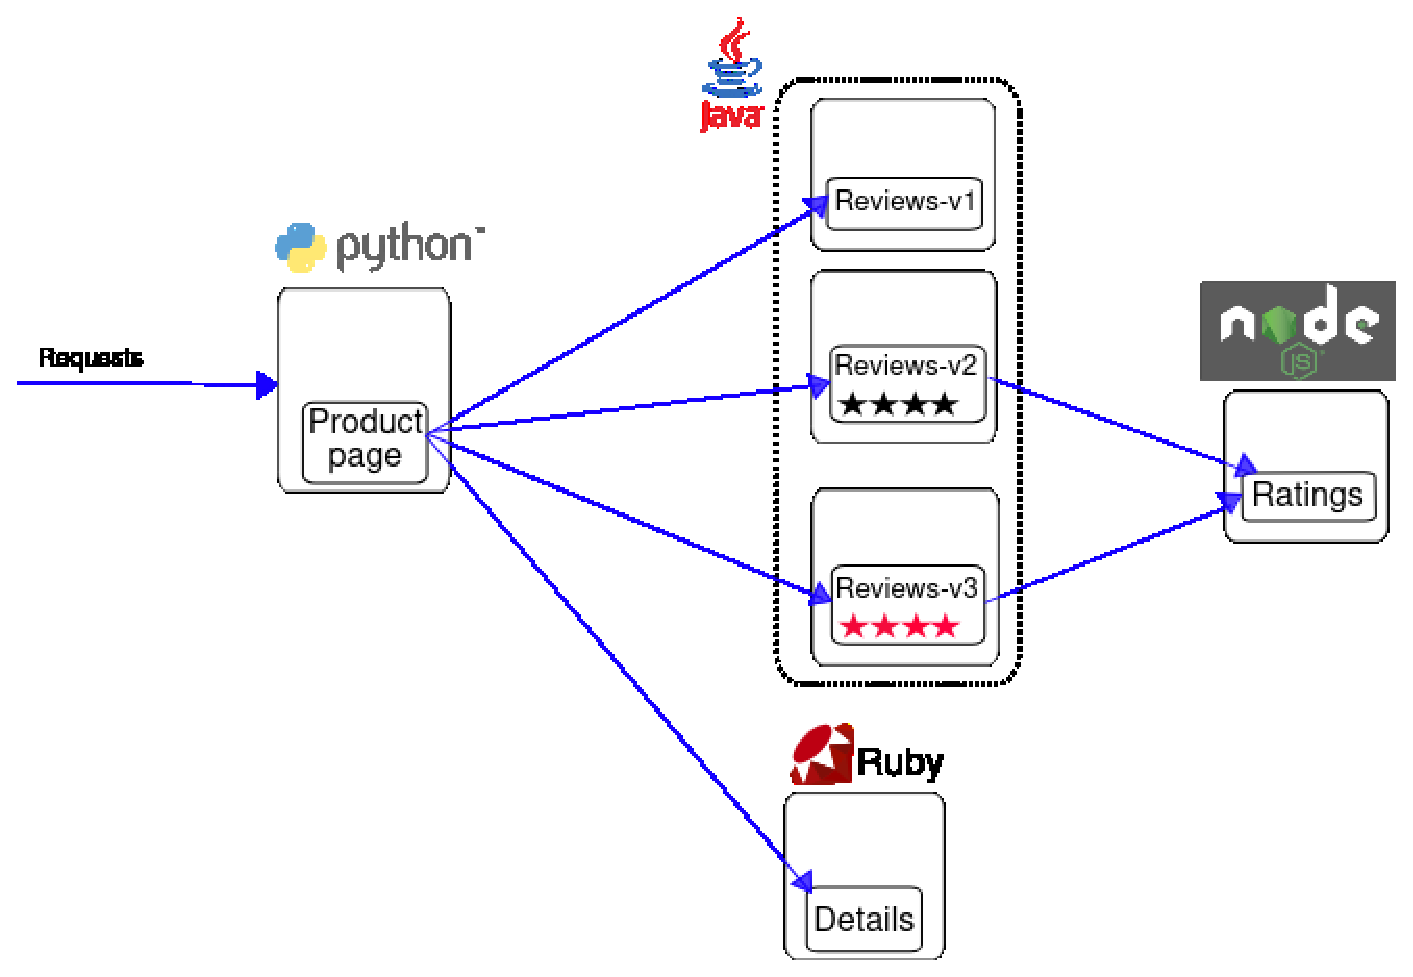
\includegraphics[scale=0.3]{imgs/bookinfo.eps}

\subsection{Installing Istio}
In this exercise, you'll install Istio in your Kubernetes cluster.
Installation and configuration are from this installation guide: \footnotesize\url{https://istio.io/latest/docs/setup/getting-started/}. \\

\normalsize

\textbf{Important Note:} While Minikube can run with as little as 2GB of RAM, Istio is resource-intensive and typically requires at least 16GB of RAM for optimal performance. Due to these high resource requirements, you may experience unexpected behavior or performance issues when running Istio on a system with limited resources. Keep this in mind as you proceed with the exercises. \\

\textbf{Steps:}
\begin{enumerate}
    \item \textbf{Install Istio CLI:}
    \begin{lstlisting}
curl -L https://istio.io/downloadIstio | sh -
export PATH="$PATH:/path/to/istio/bin/folder"  # REPLACE the path with the path you downloaded to, specifically the istio bin folder.
    \end{lstlisting}

    \item \textbf{Install Istio in the Cluster:}
    \begin{lstlisting}
istioctl install --set profile=demo -y  # if something fails, re run the command
    \end{lstlisting}
    This command installs Istio with the default configurations. Make sure that nothing fails, otherwise you have to rerun the command.

    \item \textbf{Label the default namespace for Istio injection:}
    \begin{lstlisting}
kubectl label namespace default istio-injection=enabled
    \end{lstlisting}
    This command adds add a namespace label to instruct Istio to automatically inject Envoy sidecar proxies when we will deploy the various applications later.
\end{enumerate}

\subsection{Exercise 1: Deploying and Configuring the Bookinfo App}

In this exercise, you will deploy the Bookinfo sample application to your Istio-enabled Kubernetes cluster and configure it for external access and traffic management. You can refer to the detailed guide at \footnotesize\url{https://istio.io/latest/docs/examples/bookinfo/}. \\

\normalsize
\textbf{Steps:}
\begin{enumerate}
    \item \textbf{Deploy the Bookinfo application:}
    \begin{lstlisting}
cd /path/to/istio
kubectl apply -f samples/bookinfo/platform/kube/bookinfo.yaml
    \end{lstlisting}
    This command deploys all four services and their respective versions used in the Bookinfo application.

    \item \textbf{Verify that all services and pods are running:}
    \begin{lstlisting}
kubectl get services
watch kubectl get pods  # Watch as the pods initialize (Ctrl+C to exit)
    \end{lstlisting}
    Ensure that all services (details, productpage, ratings, reviews) are listed and their respective pods are in the Running state. \textbf{Note}: It might take a few minutes for all the pods to be up!!

    \item \textbf{Confirm the Application is Running:}
    \begin{lstlisting}
# Execute a command in the 'ratings' container of the pod with the label 'app=ratings'
kubectl exec "$(kubectl get pod -l app=ratings -o jsonpath='{.items[0].metadata.name}')" -c ratings -- \
    curl -sS productpage:9080/productpage | grep -o "<title>.*</title>"

# Note: If copying from here, replace ` with normal quotes. It's advisable to paste this command into a text editor for any necessary adjustments.
    \end{lstlisting}

    This will perform a request starting from ratings pod to productpage pod. You should see output indicating that the application is running:
    \begin{lstlisting}
<title>Simple Bookstore App</title>
    \end{lstlisting}

    \item \textbf{Create a Gateway for external access:}
    
    To inspect the Istio ingress gateway's configuration, use the following:
    \begin{lstlisting}
kubectl describe svc -n istio-system istio-ingressgateway
    \end{lstlisting}
    If you scroll down, you will see (among all the others) output very similar to this:
    \begin{lstlisting}
Port:                     http2  80/TCP
TargetPort:               8080/TCP
NodePort:                 http2  30710/TCP
Endpoints:                10.244.0.160:8080
  \end{lstlisting}
    Here, the external port 80 (internally it's port 30710 in this case, it can vary, but this port is not important) is redirected to port 8080. 
    
    Now, we need to map port 8080 to the Bookinfo Gateway: \\
    in \texttt{samples/bookinfo/networking/bookinfo-gateway.yaml}, under the 'Gateway' resource type, there is the configuration which defines the port used by the Bookinfo Gateway:
    
    \begin{lstlisting}
port:
  number: 8080
  name: http
    \end{lstlisting}

    In the same file, the `VirtualService` resource configuration specifies that traffic matching some URL paths should be routed to port 9080 on the `productpage` service (otherwise, it will be a 404 error):
\begin{lstlisting}
http:
- match:
  - uri:
      exact: /productpage
  - uri:
      prefix: /static
  - uri:
      exact: /login

% ... etc etc

  route:
  - destination:
      host: productpage
      port:
        number: 9080
\end{lstlisting}

    \textbf{So finally, let's apply the rules:}
    \begin{lstlisting}
kubectl apply -f samples/bookinfo/networking/bookinfo-gateway.yaml
    \end{lstlisting}
    \textbf{So to be clear:} this command will configure the Istio ingress gateway to handle external ingress traffic directed to port \texttt{80} and to route it internally to port \texttt{8080}. The traffic is then managed by the Bookinfo Gateway, which routes it to the \texttt{productpage} service on port \texttt{9080}. \\The \texttt{samples/bookinfo/networking/bookinfo-gateway.yaml} configuration has 'Gateway' and 'VirtualService' rules which specify these settings of ports and URLs for routing.  

    \item \textbf{Expose the Ingress Gateway:}
    \begin{lstlisting}
minikube tunnel   # You could also put '&' at the end to run in the background and keep using the same terminal
    \end{lstlisting}
    This command will expose the Istio ingress gateway, assigning it an external IP. In a test lab environment like Minikube, this IP will be the internal IP of the Istio ingress gateway itself. In a cloud environment, it would be mapped to a real external load balancer.

    \item \textbf{Determine the Ingress IP and Port:}
    \begin{lstlisting}
# Define the name and namespace of the Ingress service
export INGRESS_NAME=istio-ingressgateway
export INGRESS_NS=istio-system

# Retrieve the external IP address of the Ingress service
export INGRESS_HOST=$(kubectl -n "$INGRESS_NS" get service "$INGRESS_NAME" \
-o jsonpath='{.status.loadBalancer.ingress[0].ip}')
# Note: If copying from here, replace ` with normal quotes. It's best to paste this command into a text editor for editing.

# Retrieve the port number for the HTTP2 service
export INGRESS_PORT=$(kubectl -n "$INGRESS_NS" get service "$INGRESS_NAME" \
-o jsonpath='{.spec.ports[?(@.name=="http2")].port}')
# Note: If copying from here, replace ` with normal quotes. It's best to paste this command into a text editor for editing.

# Combine the IP address and port to form the gateway URL
export GATEWAY_URL=$INGRESS_HOST:$INGRESS_PORT

# Display the full URL for the Ingress gateway
echo $GATEWAY_URL  # This is the IP address and port of the Istio Ingress gateway pointing to our Bookinfo application.

# List all services in the 'istio-system' namespace to verify the Ingress gateway details
kubectl get service -n istio-system  # This will display all Istio services, including the Ingress gateway with its IP and exposed ports.
    \end{lstlisting}

    This retrieves the IP and port of the ingress gateway for the Bookinfo application.

    \textbf{Note:} if you are using a Crownlabs machine, to be able to access it via your local browser, you have to create an SSH tunnel with these IP and port, following the mini-guide of some page ago.

    \item \textbf{Test external access to the Bookinfo application:}
    \begin{lstlisting}
curl -s "http://${GATEWAY_URL}/productpage" | grep -o "<title>.*</title>"
    \end{lstlisting}
    The expected output is:
    \begin{lstlisting}
<title>Simple Bookstore App</title>
    \end{lstlisting}
    You can also access the application from your browser at: \url{http://$GATEWAY_URL/productpage}.
\end{enumerate}

\subsection{Exercise 2: Traffic Management}
In this exercise, you'll use Istio's Virtual Services and Destination Rules to implement traffic routing and load balancing. \\

If you want further information about Traffic Management in Istio, \\you can check out: \footnotesize\url{https://istio.io/latest/docs/concepts/traffic-management/}. \\

\normalsize

\textbf{Steps:}
\begin{enumerate}
    \item \textbf{Define available versions with Destination Rules:}
    
    Before you can use Istio to control the routing of different versions of the Bookinfo application, you need to define these versions using Destination Rules. Run the following command to create default destination rules for all Bookinfo services:    
    \begin{lstlisting}
kubectl apply -f samples/bookinfo/networking/destination-rule-all.yaml
    \end{lstlisting}
    Allow a few moments for the Destination Rules to propagate. In Istio, \texttt{DestinationRules} manage traffic to specific versions of a service based on pod labels. 
    
    For example, the part related to `reviews` service:
    \begin{lstlisting}
apiVersion: networking.istio.io/v1alpha3
kind: DestinationRule
metadata:
  name: reviews
spec:
  host: reviews
  subsets:
  - name: v1
    labels:
      version: v1
  - name: v2
    labels:
      version: v2
  - name: v3
    labels:
      version: v3
        \end{lstlisting}
    Here, the `subsets` field defines three versions (v1, v2, v3) of the `reviews` service based on the labels `version: v1`, `version: v2`, and `version: v3`, respectively.
    
    These version labels are defined in the Kubernetes Deployment manifests: \\\texttt{samples/bookinfo/platform/kube/bookinfo.yaml} that we deployed at the beginning.

    \item \textbf{Verify Destination Rules:}
    To inspect the Destination Rules that have been applied, use:
    \begin{lstlisting}
kubectl describe destinationrules
    \end{lstlisting}
    You can visit with browser the \url{http://$GATEWAY_URL/productpage} and if you refresh several times you'll see at the bottom that can appear different kind of reviews: no stars (v1), black stars (v2) and red stars (v3).


    \item \textbf{Route all traffic to version v1:} 
    Create a Virtual Service to route all traffic to v1 of each microservice by running:
    \begin{lstlisting}
kubectl apply -f samples/bookinfo/networking/virtual-service-all-v1.yaml
    \end{lstlisting}
    A `VirtualService` in Istio defines routing rules for traffic within the mesh. 
    
    In particular, the `hosts` and `http` fields in the configuration file specify which traffic the routing rules apply to; the `route` section determines where the traffic is directed, in this case to the `v1` subset of the specified service, that as we said, were defined thanks the Destination Rule file \texttt{samples/bookinfo/networking/destination-rule-all.yaml}.

    \item \textbf{Display defined routes:} 
    To view the current Virtual Services and their configurations, use:
    \begin{lstlisting}
kubectl describe virtualservices
    \end{lstlisting}
    Verify the routing by accessing the application multiple times. You should only see reviews with no stars (v1).

    If you see also the stars, this means that something is off in Istio. I advice you to delete the cluster and reinstall istio so restart from the Part 2 of this lab. Unfortunately it can happen (expecially in low spec environments) that something does not work well.

    \item \textbf{Remove the previous Virtual Service rule:} 
    Delete the Virtual Service rule that routes all traffic to v1 with:
    \begin{lstlisting}
kubectl delete -f samples/bookinfo/networking/virtual-service-all-v1.yaml
    \end{lstlisting}

    \item \textbf{Implement weighted routing:} 
    Now simulate a more realistic scanario, we can think about v1 as the most lightweight service, while v3 the heaviest, so we want to forward the most of the traffic to v1, and smaller parts to v2 and v3. Let's route 50\% of the traffic to v1 review service, 30\% to v2 and 20\% to v1. Apply this configuration (don't copy-paste from PDF, but instead copy from the file in '\texttt{yamls}' folder called '\texttt{istio-weighted-routing.yaml}'):
    \begin{lstlisting}
# Here instead of applying from a file, we do it via stdin. Just to change.
kubectl apply -f - <<EOF
apiVersion: networking.istio.io/v1alpha3
kind: VirtualService
metadata:
  name: reviews
spec:
  hosts:
    - reviews
  http:
  - route:
    - destination:
        host: reviews
        subset: v1
      weight: 50
    - destination:
        host: reviews
        subset: v2
      weight: 30
    - destination:
        host: reviews
        subset: v3
      weight: 20
EOF
    \end{lstlisting}

    \item \textbf{Observe traffic distribution:} 
    Access the application multiple times. You should now see that the most of the time there are no stars (so version 1 reviews).
    
    \item \textbf{Delete the Virtual Service rule:} 
    Another way to delete a resource, is to delete it by type of resource (virtualservice) and name of rule (`reviews`, as indicated by the metadata-name above).
    \begin{lstlisting}
kubectl delete virtualservice reviews
    \end{lstlisting}
\end{enumerate}

\subsection{Exercise 3: mTLS}
In this exercise, you'll implement mutual TLS authentication between services using Istio's security features.

For further information, you can check the official documentation: \\
\footnotesize\url{https://istio.io/latest/docs/tasks/security/authentication/mtls-migration/}.

\normalsize
By default, Istio operates in 'PERMISSIVE' mode. In this mode, an Istio-injected service (a service with an Envoy sidecar) can accept both plaintext traffic from services that are not injected and mutual TLS traffic from other services that are injected. To force services in the service mesh to only communicate with Istio-injected services, you need to apply 'STRICT' mode. \\

\textbf{Steps:}
\begin{enumerate}
    \item \textbf{Enable mutual TLS for the entire mesh:}
    This will apply to any namespace with Istio-injected pods. The file is as usual in '\texttt{yamls}' folder, named '\texttt{mTLS-strict.yaml}'... copy from there.
    \begin{lstlisting}
kubectl apply -f - <<EOF
apiVersion: "security.istio.io/v1beta1"
kind: "PeerAuthentication"
metadata:
  name: "default"
  namespace: "istio-system"
spec:
  mtls:
    mode: STRICT
EOF    
\end{lstlisting}

\item \textbf{Verify that mutual TLS is enabled} looking for 'PeerAuthentication' resources (\texttt{STRICT} means having mutual TLS for all the workloads of the namespace istio-system, so basically all your istio enabled mesh):
\begin{lstlisting}
kubectl describe peerauthentication --all-namespaces
\end{lstlisting}

Next, retrieve the IP address of the `productpage` service or pod using the following commands:

\begin{lstlisting}
# Retrieve the service cluster IP of the 'productpage' service
kubectl get svc -n default

# Or:

# Retrieve the pod IP of the 'productpage' pod
kubectl get pod -n default -o wide
\end{lstlisting}

Alternatively, you can use a web dashboard to find the IPs. Remember, the IP you are looking for is the internal cluster IP, \textbf{NOT} the external `GATEWAY\_URL` used for ingress. We are testing mutual TLS (mTLS) \textbf{within} the Istio-injected cluster.

Once you have the IP, try to access the service:

\begin{lstlisting}
# Using the service cluster IP
wget -qO- http://PRODUCTPAGE_SERVICE_CLUSTER_IP:9080/productpage

# Using the pod IP
wget -qO- http://PRODUCTPAGE_POD_IP:9080/productpage
\end{lstlisting}

If mutual TLS is correctly configured, the request from a pod without the Istio sidecar should fail, as it lacks the required certificates for mTLS. To verify the mTLS configuration, you can also delete the previous `PeerAuthentication` rule with an appropriate `kubectl` command.
\begin{lstlisting}
kubectl delete peerauthentication default -n istio-system
    \end{lstlisting}
    If needed, delete the pod and create it again:
    \begin{lstlisting}
kubectl delete pod legacy-app -n legacy
kubectl run legacy-app --image=busybox -n legacy --rm -it -- /bin/sh
    \end{lstlisting}
    After recreating the pod, retry accessing the service. It should succeed if mutual TLS is not enforced.

\end{enumerate}

\subsection{Exercise 4: Observability}
In this exercise, you'll explore Istio's observability features, including graphical visualization, monitoring and tracing.

For more information I suggest to check out the official doc: 
\footnotesize
\begin{itemize}
  \item \url{https://istio.io/latest/docs/tasks/observability/kiali/}
  \item \url{https://istio.io/latest/docs/tasks/observability/metrics/using-istio-dashboard/}
  \item \url{https://istio.io/latest/docs/tasks/observability/distributed-tracing/jaeger/} \\
\end{itemize}

\normalsize

\textbf{Steps:}
We are following this: \footnotesize\url{https://istio.io/latest/docs/setup/getting-started/#dashboard}
\normalsize
\begin{enumerate}
\item \textbf{Install Kiali, Grafana, and Jaeger:}
\begin{lstlisting}
kubectl apply -f samples/addons
kubectl rollout status deployment/kiali -n istio-system
# Note: In low-spec environments, you may encounter issues during rollout. If you really cannot solve, you can delete minikube cluster and reinstall Istio.
\end{lstlisting}

\item \textbf{Access the Kiali dashboard} to view the service mesh topology, traffic flow, and metrics.
\begin{lstlisting}
istioctl dashboard kiali &
\end{lstlisting}

\item \textbf{Generate some traffic and visualize it via Kiali}.
\begin{lstlisting}
for i in $(seq 1 10000); do curl -s -o /dev/null http://$GATEWAY_URL/productpage; done
\end{lstlisting}
Now visualize the traffic via the Traffic Graph in Kiali dashboard. Select the appropriate namespace and display options (Traffic animation is visually appealing, while Traffic rate is more concrete for understanding traffic distribution). You can manually refresh and adjust the refresh interval.
You can also check error and success rates. Also, if you apply the previous discussed routing rules you'll are able to have a visual representation of the traffic splitting as you wanted.

\begin{figure}[H]
    \centering
    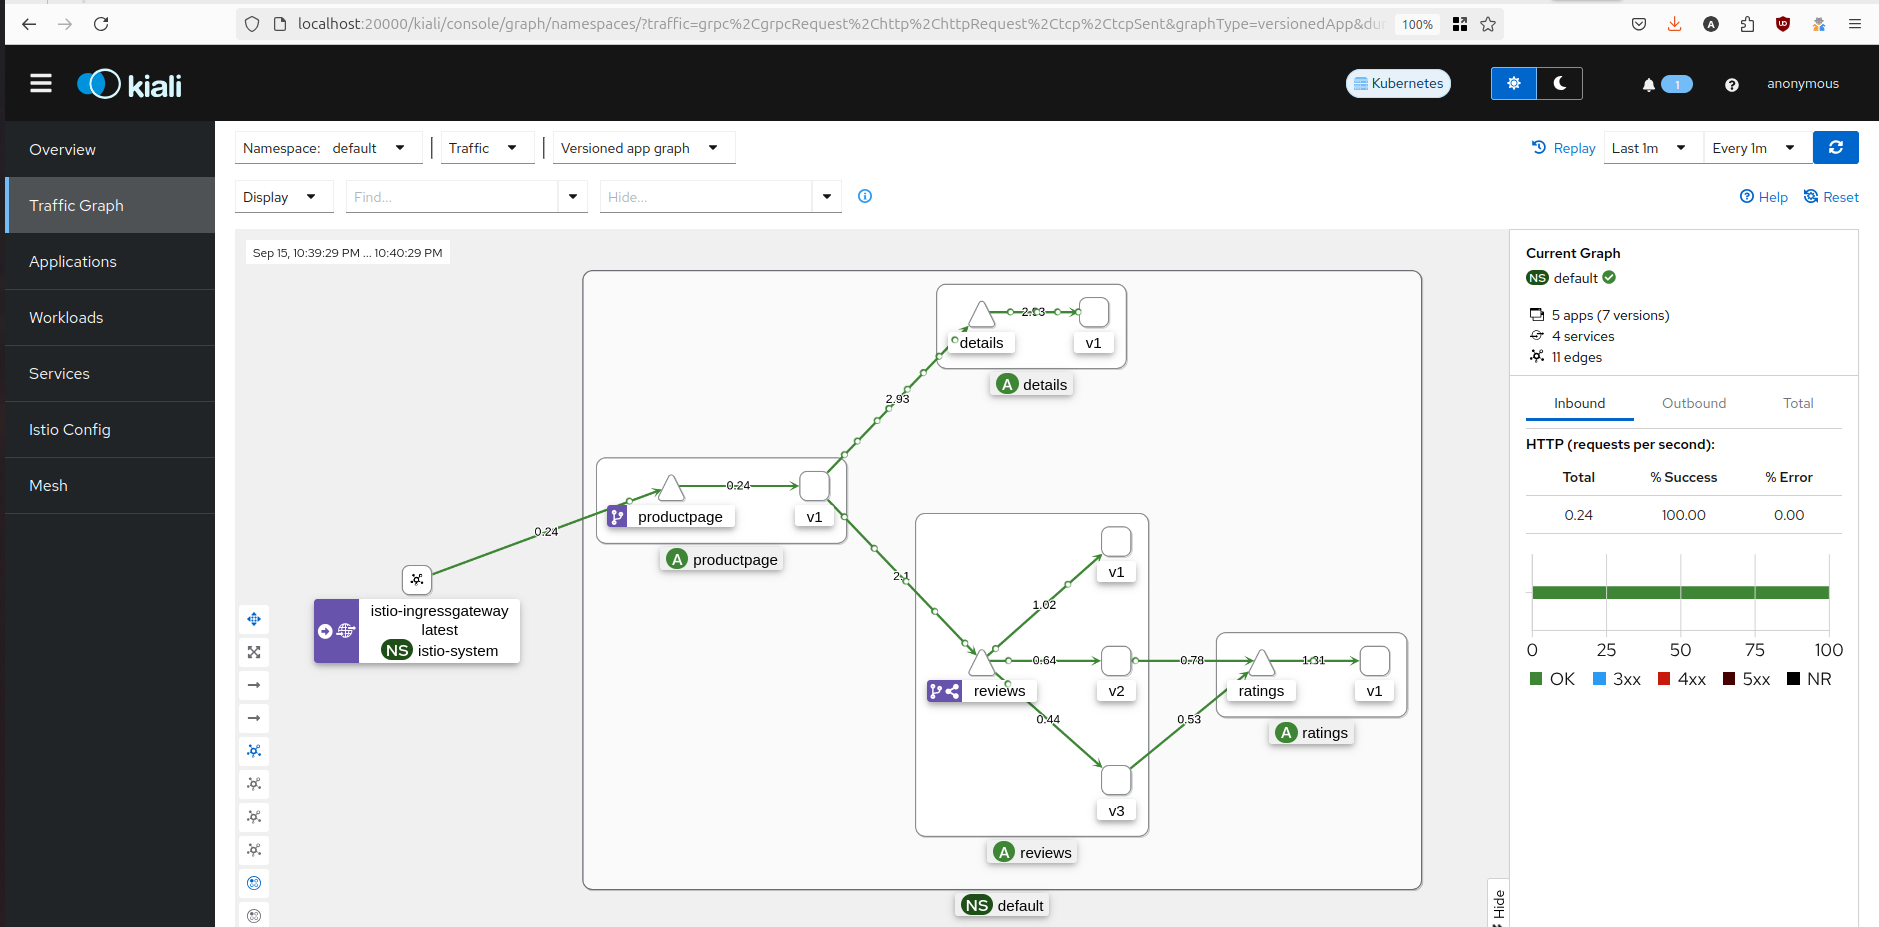
\includegraphics[width=0.7\textwidth]{imgs/kialidashboard.eps}
    \caption{Kiali Web Dashboard}
\end{figure}

\item \textbf{Access Grafana dashboard} for metrics visualization:
\begin{lstlisting}
istioctl dashboard grafana &
\end{lstlisting}
In Grafana, view the pre-built dashboards metrics for Istio, which provide insights into CPU, memory usage, and network traffic within the service mesh. Navigate to the dashboard labeled \texttt{istio} and try them. Generate traffic as mentioned above to see these metrics in action.

\begin{figure}[H]
    \centering
    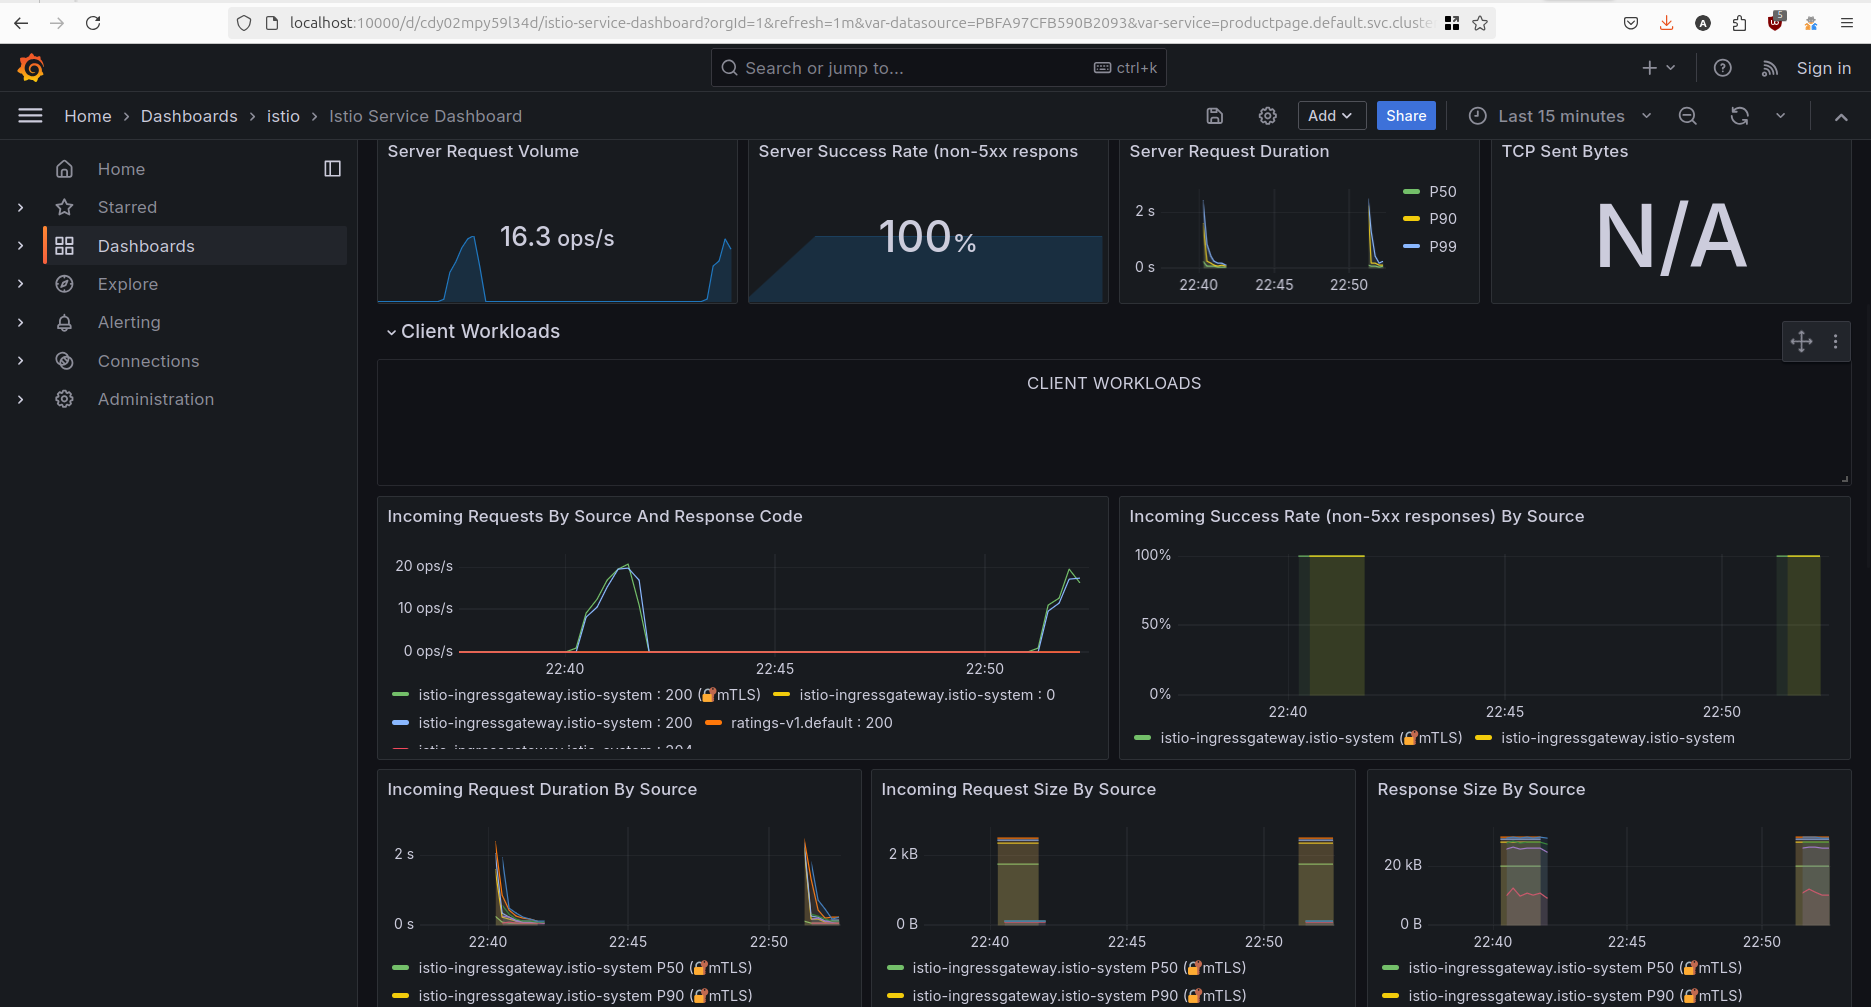
\includegraphics[width=0.7\textwidth]{imgs/grafanadashboard.eps}
    \caption{Grafana Web Dashboard}
\end{figure}

\item \textbf{Access Jaeger dashboard} for distributed tracing:
\begin{lstlisting}
istioctl dashboard jaeger &
\end{lstlisting}
In the Jaeger UI, select a service to view traces. Traces are made up of spans, which represent individual operations within a "full" request. This allows you to understand the request flow and latency/faults across different microservices. The Istio service mesh integrates tracing via the Envoy sidecar proxy, although the application must include specific headers to correlate spans into a single trace.

Note: if you don't see any traces, it might be a bug: \footnotesize\url{https://github.com/orgs/jaegertracing/discussions/4687} \footnotesize\url{https://github.com/istio/istio/issues/8709}
\end{enumerate}

\normalsize

\newpage

\section{Comparison of Network Policies and Service Meshes}

\subsection{Network Policies vs. Service Meshes}
\textbf{Network Policies:}
\begin{itemize}
\item \textbf{Pros:} 
\begin{itemize}
    \item Native Kubernetes resource, lightweight, and simple to implement.
    \item Provides basic traffic control at L3/L4, then efficient.
\end{itemize}
\item \textbf{Cons:} 
\begin{itemize}
    \item Limited to L3/L4 traffic control; lacks advanced features such as mTLS, fine-grained traffic management, and observability.
    \item Does not handle client-side load balancing or circuit breaking.
\end{itemize}
\end{itemize}

\textbf{Service Meshes:}
\begin{itemize}
\item \textbf{Pros:}
\begin{itemize}
    \item Advanced traffic management, client-side load balancing (which is more effective and scalable than k8s one), and circuit breaking (to prevent application overload and handle failures more gracefully).
    \item Security improved with mTLS for secure service-to-service communication, and it's very easy to enable it, without manually handle certificates etc.
    \item Observability and tracing out-of-the-box, without modifying application code or make application code heavier.
\end{itemize}
\item \textbf{Cons:} 
\begin{itemize}
    \item Adds complexity and overhead (requires deployment and managing of sidecar proxies (e.g., Envoy which is L7) in each pod), potentially increasing CPU consumption by 20-30\%.
\end{itemize}
\end{itemize}

\subsection{Best Practices and Considerations}
\begin{itemize}
\item Use Network Policies as a first line of defense for controlling basic pod communication.
\item Implement a Service Mesh for bigger architectures requiring more resilience and advanced features like mTLS, fine-grained traffic management, observability. \\\\\\\\
\end{itemize}

\section{Troubleshooting}

When working with Kubernetes, Network Policies, and Service Meshes, you may encounter issues. Here are some useful commands and strategies for troubleshooting:

\subsection{Useful Commands}

\begin{enumerate}
\item \textbf{View events} across all namespaces, sorted by creation timestamp, excluding normal events:
\begin{lstlisting}
kubectl get events --all-namespaces --sort-by=.metadata.creationTimestamp | grep -v 'Normal'    # where -v Normal excludes normal events and only shows other useful one, like warning
\end{lstlisting}
This command helps identify any warnings or errors that have occurred in your cluster.

\item \textbf{View all pods} across all namespaces with additional details:
\begin{lstlisting}
kubectl get pods --all-namespaces -o wide
\end{lstlisting}
This provides a comprehensive view of all pods, including their status and the nodes they're running on.

\item \textbf{View logs} for a specific pod:
\begin{lstlisting}
kubectl logs <pod-name> -n <namespace>
\end{lstlisting}
Replace \texttt{<pod-name>} with the name of the pod and \texttt{<namespace>} with the namespace it's in. This can help diagnose issues specific to a particular pod.
\end{enumerate}

\subsection{NetworkPolicy and Service Mesh Troubleshooting Strategies}

\begin{itemize}
\item \textbf{Verify Network Policies:} Check policies with \texttt{kubectl describe networkpolicy --all-namespaces}. To test if a Network Policy is causing issues, you can temporarily delete it using \texttt{kubectl delete networkpolicy <policy-name> -n <namespace>}.

\item \textbf{Istio Troubleshooting:} Run \texttt{istioctl proxy-status} to check for stale states that indicate communication issues. For broader configuration checks, use \texttt{istioctl analyze} optionally specifying a namespace with \texttt{-n}.

\item \textbf{Service Mesh Observability:} Use Kiali, Grafana and Jaeger to diagnose issues in your service mesh.
\end{itemize}

% \section{Additional Resources}
% \begin{itemize}

% \end{itemize}

\end{document}